% https://tex.stackexchange.com/a/411616
\documentclass{beamer}

\usepackage{tikz}
\usetikzlibrary{angles}

\pgfdeclarelayer{background}
\pgfdeclarelayer{foreground}
\pgfsetlayers{background,main,foreground}

\usetikzlibrary{overlay-beamer-styles}

\begin{document}
\begin{frame}

\hfill 
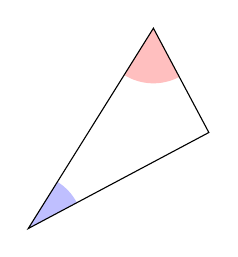
\begin{tikzpicture}

\draw[scale=1.5,rotate=118] (0,0) coordinate (A)
        --++(1,0) coordinate (B)
        --++(120:2) coordinate (C)
        --cycle ;

\begin{pgfonlayer}{background}
\draw pic[%
    semithick,
    fill=blue!25,
    angle radius=.7cm,
    visible on=<+(1)->
    ] {angle=A--C--B} ;
\draw pic[%
    semithick,
    fill=red!25,
    angle radius=.7cm,
    visible on=<+->
    ] {angle=C--B--A} ;
\end{pgfonlayer}

\end{tikzpicture}\hfill\strut
\end{frame}
\end{document}
